\chapter{Mating Like to Like}
\label{cha:Lush_Chapter_27}
\index{Assortive mating|(}
\index{Mating like to like|(}

Although many writings on animal breeding stress the importance
of mating like to like, it is usually selection which is being discussed.
The familiar recommendation to ``breed the best to the best'' usually
implies that the worst (and the mediocre as far as numbers will permit)
are to be discarded. That would be selection, whereas mating like to
like would require also the mating of the worst to the worst and the
mediocre to the mediocre --- at least among those selected to be parents.

Actually some selection is always practiced; that is, the different
types are not permitted to reproduce at equal rates. The nearest actual
approach to mating like to like without selection occurs in breeds
where there is a marked disagreement about the ideal type, some breeders
working toward one goal and some toward another. So far as
concerns those traits on which there is disagreement, these cases show
some approach to the mating of like to like in the breed as a whole,
although in each individual herd the practice is merely selection. There
is a little of this at all times in all breeds because some breeders emphasize
certain characteristics more and other characteristics less than other
breeders do. Also a breeder who uses more than one sire at a time might,
if he chooses, mate the best sire to the best females, the second best sire
to the second best group of females, etc., until finally the poorest sire
among those he uses will be left for mating to the poorest bunch of
females which he keeps. This would be mating like to like within the
selected group. By contrast he might try to balance the groups of
females so that the mates of each sire would be about equal to the mates
of every other sire in average merit. This he might well do if his primary
object was an accurate progeny test of the sires. Or he might mate
the best male to the poorest group of females he kept, the second best
male to the next to the poorest group of females, etc. That would be
mating unlikes within the group selected to be parents. That is the subject
of the next chapter. ``Best'' and ``worst'' might describe net merit
or, for one characteristic at a time, we could be more specific by using
such terms as: largest or smallest, coarsest or most refined, most active
or most sluggish, darkest or lightest, etc.

These illustrations will show how any given intensity of selection
may be accompanied by any intensity of mating like to like, ranging
from almost perfect positive through random mating to almost perfect
negative. To see clearly what additional would be accomplished by
superposing a system of mating like to like on a certain intensity of
selection, which would be practiced anyhow, it is simplest to consider
how mating like individuals together, regardless of pedigree, would
change a population not under selection.

The fundamental difference in principle between inbreeding and mating
like individuals together regardless of pedigree is that inbreeding is
the mating of individuals which are apt to have the same genes, while
assortive mating is the mating of individuals which tend to have
\textit{similar characteristics}, irrespective of their relationship.
Characteristics are only partly caused by the genes, and it often
happens that characteristics which appear to be the same are caused by
very different combinations of genes. To the extent that variations in
characteristics are caused by environment or by epistatic deviations
or by dominance deviations, the mating of like individuals may cause
only a slight tendency for mates to be alike in the genes they have.
That can be expressed quantitatively as follows for purely assortive
mating. If \textit{m} is the correlation between the net hereditary
values of mates, \textit{t} the correlation between the visible or
measurable characteristics of mates, and \textit{h} the correlation
between the characteristic and the net hereditary value of the same
individual, then under purely assortive mating $m = h^2t$ and
\textit{m} cannot exceed $h^2$, even if the breeder has succeeded in
getting the mates to be perfectly alike (except for sex) in all
characteristics he can see or measure. On the other hand, under
purely inbreeding systems $t = h^2m$ and \textit{t} cannot exceed
$h^2$. As a numerical example consider a moderately heritable
characteristic for which $h^2$ = .2. Under purely phenotypic
assortive mating \textit{m} could not exceed .2 even if \textit{t}
were made perfect. In actual practice it would be less. By
contrast in the first generation of full brother-sister inbreeding
\textit{m} would be .5 and \textit{t} would be only .1. The actual
consequences of phenotypic assortive mating depend largely on what
size of m really is achieved. Hence they are very slight for
characteristics moderate or low in heritability.

The example shown in Table~\ref{tbl:Lush_Table_19} deals with
variation in only one characteristic. The practical breeder must
nearly always consider many traits. He will be using only one or
at most a few sires but will have several females, no two of which
are alike, to mate to each sire. Many of the animals he might
choose to mate together are alike in some characteristics,
moderately unlike in others, and perhaps extreme opposites
in still others. If he considers many characteristics, it will
be impossible for him to achieve in all respects a high degree of
resemblance between mates. This is in addition to the general
situation, discussed in the preceding paragraph, that under
assortive mating, likeness in net hereditary values will be less
than outward likeness. In actual practice assortive mating can
rarely cause \textit{m} to have high values for any characteristic
other than net merit.

\section*{ONE PAIR OF GENES}

If only one pair of genes is involved and if there is no dominance or
other reason for mistaking hereditary values -- i.e., if \textit{h}
and \textit{t} of the next to the last paragraph each equal 1.0 -- the
results are the same as in self-fertilization. If dominance is complete
but there is no other complication, the change is in the same direction
and the final result is the same but progress is slower. If the attempt
to mate like to like is not quite perfectly successful -- i.e., if
\textit{t} is less than 1.0 or if anything other than dominance makes
\textit{h} less than 1.0 -- the population will come to equilibrium
while a few heterozygotes still remain.

\section*{TWO PAIRS OF GENES --- SIMPLEST CASE}
\index{Variation!increased by mating like to like|(}

If this mating of like to like is for a characteristic influenced by two
pairs of genes, lacking dominance and with equal effects, then we have
the situation shown in Table~\ref{tbl:Lush_Table_19} which starts with a
random breeding population in which the two pairs of genes are independent
and the two alleles of each pair are equally abundant, that is, in which
$q_A = q_B = .5$.

\begin{table}[htbp]
	\centering
	\caption{\textsc{Proportions of Each Phenotype Under a Perfectly Accurate System of Mating
Like to Like,} $q_A$ \textsc{and} $q_B$ \textsc{Remaining at .5}}
	\label{tbl:Lush_Table_19}
	\begin{tabular}{C{2cm}|C{2cm}|C{2cm}|C{2cm}|C{2cm}|C{2cm}}
		\hline
		\hline
		~			& ~			& ~			& aa{BB}	& ~			& ~		\\
		~			& ~			& aaBb		& {AA}bb	& Aa{BB}	& ~		\\
		Genotypes	& aabb		& Aabb		& AaBb		& {AAB}b	& AABB	\\
		\hline
		~			& No Plus	& 1 Plus	& 2 Plus	& 3 Plus	& 4 Plus	\\
		Phenotypes	& Genes		& Genes		& Genes		& Genes		& Genes		\\	
		\hline
		Generation:	& ~			& ~			& ~			& ~			& ~			\\
		Start		& 6.2\%		& 25.0\%	& 37.5\%	& 25.0\%	& 6.2\%		\\
		1			& 13.6\%	& 20.8\%	& 31.2\%	& 20.8\%	& 13.6\%	\\
		2			& 19.3\%	& 16.5\%	& 28.4\%	& 16.5\%	& 19.3\%	\\
		3			& 23.9\%	& 13.8\%	& 24.6\%	& 13.8\%	& 23.9\%	\\
		$\cdots$	& $\cdots$	& $\cdots$	& $\cdots$	& $\cdots$	& $\cdots$	\\
		$\cdots$	& $\cdots$	& $\cdots$	& $\cdots$	& $\cdots$	& $\cdots$	\\
		$\infty$	& 50.0\%	& 0.0\%		& 0.0\%		& 0.0\%		& 50.0\%	\\
		\hline
	\end{tabular}
\end{table}

The result is a decrease in the proportion of the intermediate
phenotypes and a corresponding increase in the two extreme phenotypes.
If the mating of like to like is perfect and is carried on forever, it
approaches as a limit the condition in which all of the genotypes have
disappeared except the two homozygous extreme ones. If the mates are
not exactly alike phenotypically, as, for example, if an occasional mistake
is made in classifying an individual, progress will be slower, and
the ultimate goal will be an equilibrium which falls short of complete
fixation of the two extreme phenotypes.

This system of breeding tends to fix the extreme types, provided
those are both outwardly and genetically extreme; but, in contrast to
inbreeding, it cannot fix intermediate types. The likeness between parent
and offspring and the likeness between full brothers increases very
rapidly, although that may not be clear from this example. The variability
of the population is greatly increased, since the population tends
to become concentrated at the two extremes.

\section*{MANY PAIRS OF GENES}
\index{Genes, number of|(}
\index{Heterozygosis|(}

Many more than two pairs of genes may affect the characteristic,
and the effects of the different pairs of genes will rarely be equal. The
more genes there are, the slower is the rate of increase in homozygosis.
The likeness of parent and offspring or of full brothers also increases at
a slower rate when n is large, although these likenesses are not nearly
as much affected by changes in gene number as is the rate of increase in
homozygosis.

\section*{GENERAL RESULTS OF MATING LIKE TO LIKE}
\index{Homozygosis|(}

Very little genuine fixation of type is ever accomplished by this system
of breeding because increase in homozygosis is dependent upon the
number of genes being very small and upon the breeder's not being
deceived by dominance, environmental effects, or epistasis.
Figure~\ref{fig:Lush_Figure_46} shows what happens to homozygosis as a
result of mating like to like. Here \textit{n} is the number of gene pairs
involved, while \textit{m} is the correlation between the net hereditary
values of mates. Both \textit{m} and \textit{n} set limits on the amount
of homozygosis which may finally be attained, and \textit{n} has a
tremendous influence on the rate at which it is attained. Only with very
high values of \textit{m} and very low values of \textit{n} can such a
breeding system alter homozygosis much. The values of \textit{m} cannot
often be high in actual practice, and \textit{n} will probably be large 
for all characteristics of much economic importance.\footnote{The fraction
of the heterozygosis of a random breeding population which will still
remain when assort1ve mating has done all can is $\dfrac{2n(1 - m)}{2n(1 - m)+m}$.
Since \textit{m} cannot exceed 1.0 (it must usually be much smaller) and
\textit{n} can be large, this fraction will rarely be much less than unity.
\textit{Genetics}, 6:153.}

\begin{figure}
	\centering
    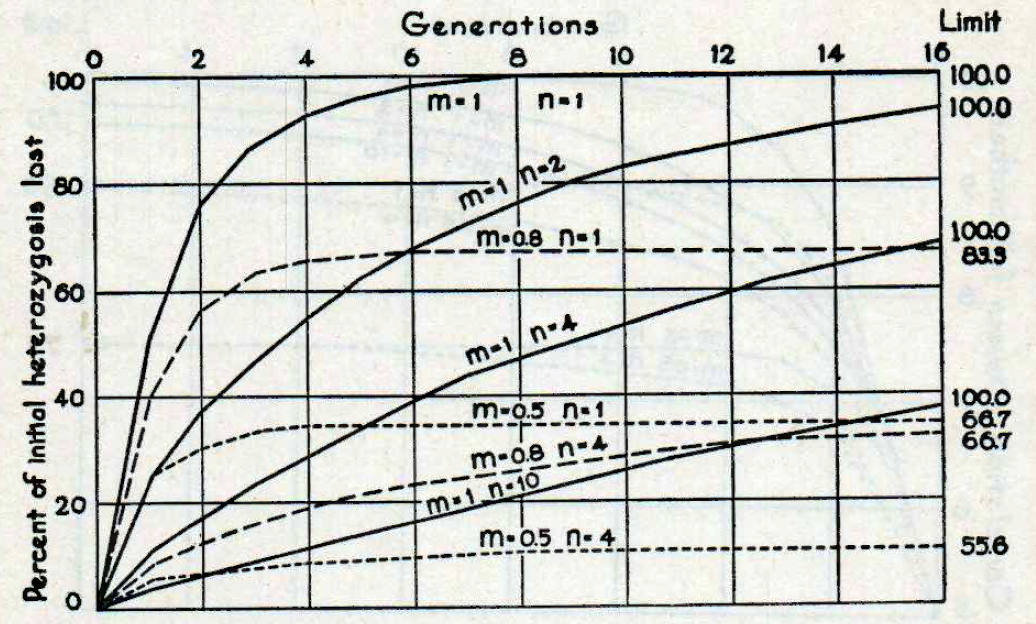
\includegraphics[width=\textwidth]{Figure_46.png}
    \caption{The percentage of initial heterozygosis which is lost by continued assortive
			 mating of various intensities, \textit{m}, and with \textit{n} pairs of equal
			 genes involved. (After Wright in \textit{Genetics}, 6:175.)}
    \label{fig:Lush_Figure_46}
\end{figure}

Mating like to like increases the resemblance of parent and offspring
very much, each individual resembling its sire not only because it
received half its inheritance from him but also because it received half
its inheritance from its dam who resembled the sire more than if mating
had been random. That is, the dam was chosen to have many genes
which produce the same kinds of effects as the sire's genes do, although
they may not be genes from the same allelic series. The limit which the
parent-offspring correlation approaches is determined by \textit{m}, large
\textit{n} merely making the approach to that limit a little slower. The
parent-offspring correlation goes far toward its limit in the first two
generations in which mating like to like is practiced.
\index{Homozygosis|)}

Figure~\ref{fig:Lush_Figure_47} shows what happens to the correlation
between full brothers under purely assortive mating in the extremely
simple case of no dominance, no epistasis, and no environmental
variations which are incorrectly discounted. The limits are determined
by \textit{m} and the only effect of large \textit{n} is to make progress
a little slower. This system of breeding has considerable effect, even
when \textit{m} is small and \textit{n} is large. The existence of
dominance and epistasis and environmental effects has the effect of making
\textit{m} lower than it need be otherwise. Environmental effects might
increase the correlations if these effects tended to be the same for brothers.
\index{Genes, number of|)}
\index{Heterozygosis|)}

A high degree of resemblance between parent and offspring and a
high degree of resemblance between full brothers seem to indicate that
the breeder is gaining control over his material, but that is partly contradicted
by the fact that there is little increase in real homozygosis.
This has long been recognized in a general way by breeders in the confidence
they have in the mating of like to like as a means of getting the
kind of herd they want, but again and again the more experienced
among them express the idea that inbreeding is really necessary if type
is to be ``fixed''

\begin{figure}
	\centering
    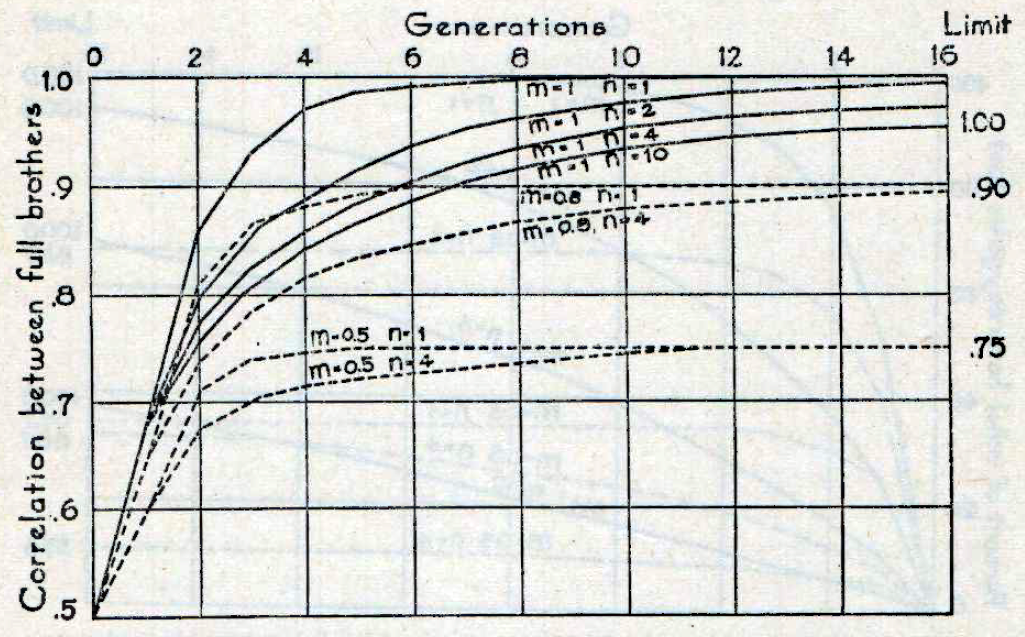
\includegraphics[width=\textwidth]{Figure_47.png}
    \caption{The correlations between brothers in successive generations
    		 under different degrees, \textit{m}, of assortive mating and
    		 with \textit{n} pairs of genes involved. (After Wright in
    		 \textit{Genetics}, 6:170.)}
    \label{fig:Lush_Figure_47}
\end{figure}

Mating like to like is one of the most powerful tools which breeders
have for creating extreme diversity in a population. Inbreeding tends
to fix intermediate families as well as extreme ones and thereby tends
to double the additive genetic variance of the population. But mating
like to like tends to scatter the population toward the two opposite
extremes of each characteristic for which it is practiced. For example,
assortive mating for stature within most local races of man is enough to
make the standard deviation about 20 or 25 per cent larger than it
would be if mating were entirely random with respect to stature. If the
characteristic is highly enough hereditary that \textit{m} in assortive
mating can rise above .5, mating like to like can make the standard
deviation in an unselected population larger than the most extreme
inbreeding can.\footnote{\textit{Genetics}, 6:154.} In each individual
herd the mating of like to like will usually be accompanied by selection
which will discard one or the other extreme. If all breeders select
toward the same ideal, this will not change the variability
of the whole breed any more than selection changes the variability
within a single herd. But if the breeders disagree markedly about the
ideal and some of them discard animals which other breeders think are
very desirable, this process can easily produce a lack of uniformity, in
the breed as a whole, so pronounced that everyone familiar with the
breed will be aware of it. Examples which have shown some tendency in
that direction are: ``Island type'' and ``American type'' in Jerseys;
``hot bloods'' and ``big types'' in Poland-Chinas. Even when all breeders
work toward the same ideals, a little of this herd heterogeneity within a
breed will arise because some breeders will try harder than others or
will be financially able to outbid others for the animals thought best.
Such inequality of striving toward the same ideal produces to a very
mild degree something of the same results as a divergence of ideals.
The changes brought about by purely assortive mating are temporary.
If there has been no accompanying selection, the population
returns far toward its initial condition in the very first generation after
random mating is resumed. In actual practice there will, of course, have
been some selection; and that is apt to have changed gene frequency
enough that the population will never return exactly to its initial
condition.
\index{Variation!increased by mating like to like|)}

\section*{SUMMARY}

Mating like to like has almost no effect on homozygosis except in
very simple and rare genetic circumstances.

Mating like to like immediately increases the resemblance between
parent and offspring and between full brothers.

Mating like to like comes near to the full limit of its effects within a
very few generations after it is begun.

Mating like to like tends to scatter a population toward the two
extremes with respect to each character for which such mating is practiced.
It, therefore, greatly increases the variability of the population if
both extremes are kept and heritability is high.

In actual practice mating like to like is always accompanied by
selection.

The effects of mating like to like disappear almost at once when random
mating is resumed, except as the accompanying selection may have
made some permanent changes in gene frequency.

\section*{REFERENCES}

\begin{hangparas}{0.5in}{1}%
Wright, Sewall. 1921. Systems of mating. {III}. Assortive mating, based on somatic
resemblance. Genetics, 6:144--61. (See also pp. 167--78.)
\end{hangparas}
\index{Mating like to like|)}